% Session 7 -- tensor diagram notation, the MPS, and the MPO/truncation step.
% Placement: sec. "Tensor diagrams: notation for networks and operators", after the
% Rendered by figures/blender/s07f04_tensordiagram.py, labels in figures/overlays/s07f04_tensordiagram.tex.
\begin{aqmfigure}{fig:s07:tensors}{The graphical notation, and the MPS ansatz drawn in it. (a) A
tensor is a block and each of its indices is a leg, so a scalar has no leg, a vector has one leg, a
matrix has two, and so on. Joining two legs means summing over the shared index. (b) The exact
coefficient tensor of (7.4) is a single object with one leg per site, and it contains $2^L$
independent numbers. The matrix product state (7.5) replaces it with a chain of small tensors. Each
of them has one physical leg pointing down and virtual legs of dimension $M$ that link it to its
neighbours, for a total of $\sim 2LM^2$ numbers, so the exponential growth is replaced by a chain
that grows linearly. (c) An operator, in particular the Hamiltonian, becomes a matrix product
operator, the darker row, with two physical legs per site. To apply it to a state we join the
diagrams along the shared physical legs and contract them, which multiplies the two bond dimensions.
A singular value decomposition that keeps only the largest singular values then truncates the result
back to a usable $M$. This truncation is the core of every MPS algorithm, including DMRG.}
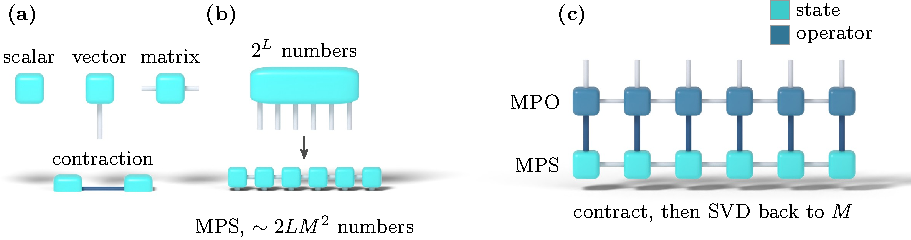
\includegraphics{figures/pdf/s07f04_tensordiagram.pdf}
\end{aqmfigure}
